\section{Supplementary material}

\subsection{Descriptive statistics}

General descriptive statistics of patients in the retrieved SSNAP data set is shown in tables \ref{tab:hospital_stats_1} and \ref{tab:hospital_stats_2}.

\small
\renewcommand{\arraystretch}{1.3}
\begin{longtable}{p{7cm} p{1cm} p{0.8cm} p{0.8cm} p{0.8cm} p{0.8cm} p{0.8cm} p{0.8cm} p{0.8cm} p{0.8cm}}
\caption{Descriptive statistics for all patients arriving at each stroke team. The table shows summary statistics across all stroke teams.}\\
\toprule
\endhead
Statistic & Stroke teams & mean & Std Dev & min & 25\% & 50\% & 75\% & max\tabularnewline
\midrule
Yearly admissions & 119 & 509 & 208 & 95 & 372 & 489 & 627 & 1183\tabularnewline
Age (mean) & 119 & 74 & 2 & 65 & 73 & 75 & 76 & 78\tabularnewline
Proportion aged 80+ & 119 & 0.40 & 0.06 & 0.20 & 0.36 & 0.40 & 0.44 & 0.51\tabularnewline
Proportion male & 119 & 0.53 & 0.02 & 0.47 & 0.51 & 0.53 & 0.55 & 0.60\tabularnewline
Prior disability (mRS, mean) & 119 & 1.02 & 0.25 & 0.29 & 0.87 & 1.03 & 1.21 & 1.60\tabularnewline
Proportion prior disability (mRS) 0-2 & 119 & 0.81 & 0.05 & 0.67 & 0.78 & 0.81 & 0.84 & 0.97\tabularnewline
Proportion ischaemic stroke & 119 & 0.88 & 0.02 & 0.83 & 0.86 & 0.88 & 0.89 & 0.93\tabularnewline
Stroke severity (NIHSS, mean) & 119 & 7.0 & 1.0 & 4.6 & 6.3 & 7.2 & 7.8 & 9.1\tabularnewline
Proportion with known onset & 119 & 0.68 & 0.14 & 0.43 & 0.58 & 0.67 & 0.76 & 1.00\tabularnewline
Onset-to-arrival time (minutes, median) & 119 & 204 & 76 & 109 & 155 & 180 & 224 & 466\tabularnewline
Proportion arriving within 4 hours known onset & 119 & 0.38 & 0.06 & 0.19 & 0.34 & 0.38 & 0.43 & 0.51\tabularnewline
Proportion with precisely known onset & 119 & 0.33 & 0.11 & 0.01 & 0.28 & 0.34 & 0.39 & 0.63\tabularnewline
Proportion onset during sleep & 119 & 0.14 & 0.06 & 0.00 & 0.09 & 0.14 & 0.17 & 0.34\tabularnewline
Proportion arrive by ambulance & 119 & 0.78 & 0.07 & 0.47 & 0.76 & 0.79 & 0.82 & 0.92\tabularnewline
Call-to-ambulance arrival time (minutes, median) & 113 & 22 & 10 & 13 & 17 & 20 & 24 & 103\tabularnewline
Ambulance on scene time (median) & 113 & 31 & 3 & 20 & 28 & 31 & 33 & 41\tabularnewline
Ambulance conveyance time (minutes, median) & 113 & 18 & 5 & 10 & 15 & 17 & 21 & 37\tabularnewline
Arrival-to-scan time (minutes, median) & 119 & 53 & 21 & 13 & 39 & 51 & 63 & 129\tabularnewline
Proportion receiving thrombolysis & 119 & 0.115 & 0.034 & 0.021 & 0.092 & 0.110 & 0.136 & 0.245\tabularnewline
Scan-to-thrombolysis time (minutes, median) & 119 & 34 & 10 & 14 & 28 & 34 & 41 & 72\tabularnewline
Discharge disability (mRS, mean) & 119 & 2.641 & 0.352 & 1.361 & 2.413 & 2.699 & 2.900 & 3.320\tabularnewline
Proportion discharged mRS 0-2 & 119 & 0.524 & 0.095 & 0.293 & 0.454 & 0.522 & 0.594 & 0.799\tabularnewline
Proportion discharged mRS 5-6 & 119 & 0.195 & 0.037 & 0.095 & 0.170 & 0.198 & 0.218 & 0.287\tabularnewline
\bottomrule
\label{tab:hospital_stats_1}
\end{longtable}
\normalsize

\small
\begin{longtable}{p{7cm} p{1cm} p{0.8cm} p{0.8cm} p{0.8cm} p{0.8cm} p{0.8cm} p{0.8cm} p{0.8cm} p{0.8cm}}
\caption{Descriptive statistics for patients arriving at each stroke team, for patients arriving within 4 hours of known stroke onset. The table shows summary statistics across all stroke teams.}\\
\toprule
\endhead
Statistic & Stroke teams & mean & Std Dev & min & 25\% & 50\% & 75\% & max\tabularnewline
\midrule
Yearly admissions & 119 & 193 & 78 & 28 & 139 & 183 & 241 & 428\tabularnewline
Age (mean) & 119 & 75 & 2 & 66 & 73 & 75 & 76 & 79\tabularnewline
Proportion aged 80+ & 119 & 0.41 & 0.06 & 0.23 & 0.37 & 0.41 & 0.45 & 0.57\tabularnewline
Proportion male & 119 & 0.53 & 0.03 & 0.45 & 0.51 & 0.53 & 0.55 & 0.64\tabularnewline
Prior disability (mRS, mean) & 119 & 1.04 & 0.25 & 0.37 & 0.88 & 1.04 & 1.22 & 1.60\tabularnewline
Proportion prior disability (mRS) 0-2 & 119 & 0.80 & 0.06 & 0.66 & 0.77 & 0.81 & 0.83 & 0.95\tabularnewline
Proportion ischaemic stroke & 119 & 0.85 & 0.03 & 0.75 & 0.84 & 0.85 & 0.87 & 0.94\tabularnewline
Stroke severity (NIHSS, mean) & 119 & 8.9 & 1.1 & 6.4 & 8.2 & 9.0 & 9.7 & 11.4\tabularnewline
Proportion with known onset & 119 & 1.00 & 0.00 & 1.00 & 1.00 & 1.00 & 1.00 & 1.00\tabularnewline
Onset-to-arrival time (minutes, median) & 119 & 105 & 9 & 85 & 100 & 105 & 111 & 132\tabularnewline
Proportion arriving within 4 hours known onset & 119 & 1.00 & 0.00 & 1.00 & 1.00 & 1.00 & 1.00 & 1.00\tabularnewline
Proportion with precisely known onset & 119 & 0.62 & 0.17 & 0.02 & 0.54 & 0.66 & 0.75 & 0.91\tabularnewline
Proportion onset during sleep & 119 & 0.05 & 0.05 & 0.00 & 0.01 & 0.03 & 0.06 & 0.30\tabularnewline
Proportion arrive by ambulance & 119 & 0.89 & 0.07 & 0.54 & 0.87 & 0.91 & 0.93 & 0.98\tabularnewline
Call-to-ambulance arrival time (minutes, median) & 110 & 19 & 5 & 8 & 16 & 18 & 21 & 51\tabularnewline
Ambulance on scene time (median) & 110 & 28 & 4 & 20 & 26 & 28 & 31 & 46\tabularnewline
Ambulance conveyance time (minutes, median) & 110 & 17 & 4 & 9 & 14 & 16 & 20 & 28\tabularnewline
Arrival-to-scan time (minutes, median) & 119 & 27 & 11 & 4 & 21 & 28 & 34 & 100\tabularnewline
Proportion receiving thrombolysis & 119 & 0.293 & 0.070 & 0.111 & 0.250 & 0.282 & 0.333 & 0.534\tabularnewline
Scan-to-thrombolysis time (minutes, median) & 119 & 34 & 10 & 14 & 28 & 34 & 40 & 71\tabularnewline
Discharge disability (mRS, mean) & 119 & 2.803 & 0.353 & 1.507 & 2.609 & 2.837 & 3.039 & 3.663\tabularnewline
Proportion discharged mRS 0-2 & 119 & 0.494 & 0.094 & 0.209 & 0.424 & 0.495 & 0.554 & 0.771\tabularnewline
Proportion discharged mRS 5-6 & 119 & 0.236 & 0.045 & 0.138 & 0.208 & 0.231 & 0.256 & 0.420\tabularnewline
\bottomrule
\label{tab:hospital_stats_2}
\end{longtable}
\normalsize

\small
\begin{longtable}{p{7cm} p{1cm} p{0.8cm} p{0.8cm} p{0.8cm} p{0.8cm} p{0.8cm} p{0.8cm} p{0.8cm} p{0.8cm}}
\caption{Descriptive statistics for patients arriving at each stroke team, for patients arriving by ambulance within 4 hours of known stroke onset. The table shows summary statistics across all stroke teams.}\\
\toprule
\endhead
Statistic & Stroke teams & mean & Std Dev & min & 25\% & 50\% & 75\% & max\tabularnewline
\midrule
Yearly admissions & 119 & 173 & 74 & 15 & 125 & 163 & 227 & 400\tabularnewline
Age (mean) & 119 & 75 & 2 & 66 & 74 & 76 & 77 & 81\tabularnewline
Proportion aged 80+ & 119 & 0.43 & 0.06 & 0.24 & 0.39 & 0.43 & 0.47 & 0.62\tabularnewline
Proportion male & 119 & 0.52 & 0.03 & 0.45 & 0.51 & 0.52 & 0.54 & 0.60\tabularnewline
Prior disability (mRS, mean) & 119 & 1.10 & 0.25 & 0.46 & 0.94 & 1.09 & 1.26 & 1.66\tabularnewline
Proportion prior disability (mRS) 0-2 & 119 & 0.79 & 0.06 & 0.65 & 0.75 & 0.79 & 0.83 & 0.93\tabularnewline
Proportion ischaemic stroke & 119 & 0.85 & 0.03 & 0.75 & 0.83 & 0.85 & 0.87 & 0.94\tabularnewline
Stroke severity (NIHSS, mean) & 119 & 9.4 & 1.2 & 6.7 & 8.6 & 9.5 & 10.2 & 12.2\tabularnewline
Proportion with known onset & 119 & 1.00 & 0.00 & 1.00 & 1.00 & 1.00 & 1.00 & 1.00\tabularnewline
Onset-to-arrival time (minutes, median) & 119 & 106 & 10 & 84 & 99 & 105 & 112 & 151\tabularnewline
Proportion arriving within 4 hours known onset & 119 & 1.00 & 0.00 & 1.00 & 1.00 & 1.00 & 1.00 & 1.00\tabularnewline
Proportion with precisely known onset & 119 & 0.62 & 0.17 & 0.02 & 0.54 & 0.65 & 0.75 & 0.92\tabularnewline
Proportion onset during sleep & 119 & 0.05 & 0.05 & 0.00 & 0.01 & 0.03 & 0.06 & 0.33\tabularnewline
Proportion arrive by ambulance & 119 & 1.00 & 0.00 & 1.00 & 1.00 & 1.00 & 1.00 & 1.00\tabularnewline
Call-to-ambulance arrival time (minutes, median) & 110 & 19 & 5 & 8 & 16 & 18 & 21 & 51\tabularnewline
Ambulance on scene time (median) & 110 & 28 & 4 & 20 & 26 & 28 & 31 & 46\tabularnewline
Ambulance conveyance time (minutes, median) & 110 & 17 & 4 & 9 & 14 & 16 & 20 & 28\tabularnewline
Arrival-to-scan time (minutes, median) & 119 & 26 & 11 & 4 & 20 & 25 & 33 & 95\tabularnewline
Proportion receiving thrombolysis & 119 & 0.300 & 0.072 & 0.130 & 0.252 & 0.289 & 0.345 & 0.537\tabularnewline
Scan-to-thrombolysis time (minutes, median) & 119 & 34 & 10 & 13 & 27 & 33 & 40 & 73\tabularnewline
Discharge disability (mRS, mean) & 119 & 2.926 & 0.352 & 1.867 & 2.717 & 2.928 & 3.150 & 3.819\tabularnewline
Proportion discharged mRS 0-2 & 119 & 0.465 & 0.096 & 0.184 & 0.398 & 0.462 & 0.524 & 0.696\tabularnewline
Proportion discharged mRS 5-6 & 119 & 0.254 & 0.051 & 0.147 & 0.221 & 0.253 & 0.280 & 0.486\tabularnewline
\bottomrule
\label{tab:hospital_stats_3}
\end{longtable}
\normalsize


\subsection{Data}

Dataset includes the patient cohort (78,396) to make a clinical decision about whether to give thrombolysis:
\begin{enumerate}
    \item Ischaemic patients
    \item Have either/neither/both thrombolysis/thrombectomy.
    \item Not on anticoagulants.
    \item Arrive at hospital by ambulance after stroke onset.
    \item Have scan within 255 mins of stroke onset.
\end{enumerate}

\textbf{Summary of patient numbers during patient cohort creation}.
\begin{enumerate}
    \item Patients extracted (ischaemic, any/neither acute treatment, arrive at hospital by ambulance after stroke onset, have scan within 255 mins of stroke onset): 91,464
    \item Removed the 11,780 (12.9\%) patients on atrial fibrilation anticoagulants: 79,684
    \item Removed the 1,288 patients that attended hospitals with too few stroke admissions, or thrombolysis procedures: 78,396
\end{enumerate}
Of the 78,396 patient, 2,747 patients received thrombectomy, 75,649 did not.
Of the 75,649 patients not receive thrombectomy, 43,152 received thrombolysis and 32,497 did not.

The 78,396 patients attended 111 hospitals with admissions ranging from 267 to 1,414 (figure \ref{fig:admission_rate}), and thrombolysis rate ranging from 24\% to 67\%  (figure \ref{fig:thrombolysis_rate}). Of those 43,152 patients that do not receive thrombolysis (and not thrombectomy), 14\% has mRS0, 21\% have mRS1, 17\% have mRS2, 15\% have mRS3, 12\% have mRS4, 7\% have mRS5, and 13\% have mRS6 at discharge (figure \ref{fig:mrs_dist_wrt_ivt_bar}). Of those 32,497 patients that receive thrombolysis (and not thrombectomy), 15\% has mRS0, 21\% have mRS1, 18\% have mRS2, 16\% have mRS3, 12\% have mRS4, 5\% have mRS5, and 13\% have mRS6 at discharge (figure \ref{fig:mrs_dist_wrt_ivt_bar}).


\begin{figure}
    \centering
    \begin{subfigure}{.5\textwidth}
      \centering
      \captionsetup{width=.9\linewidth}
        {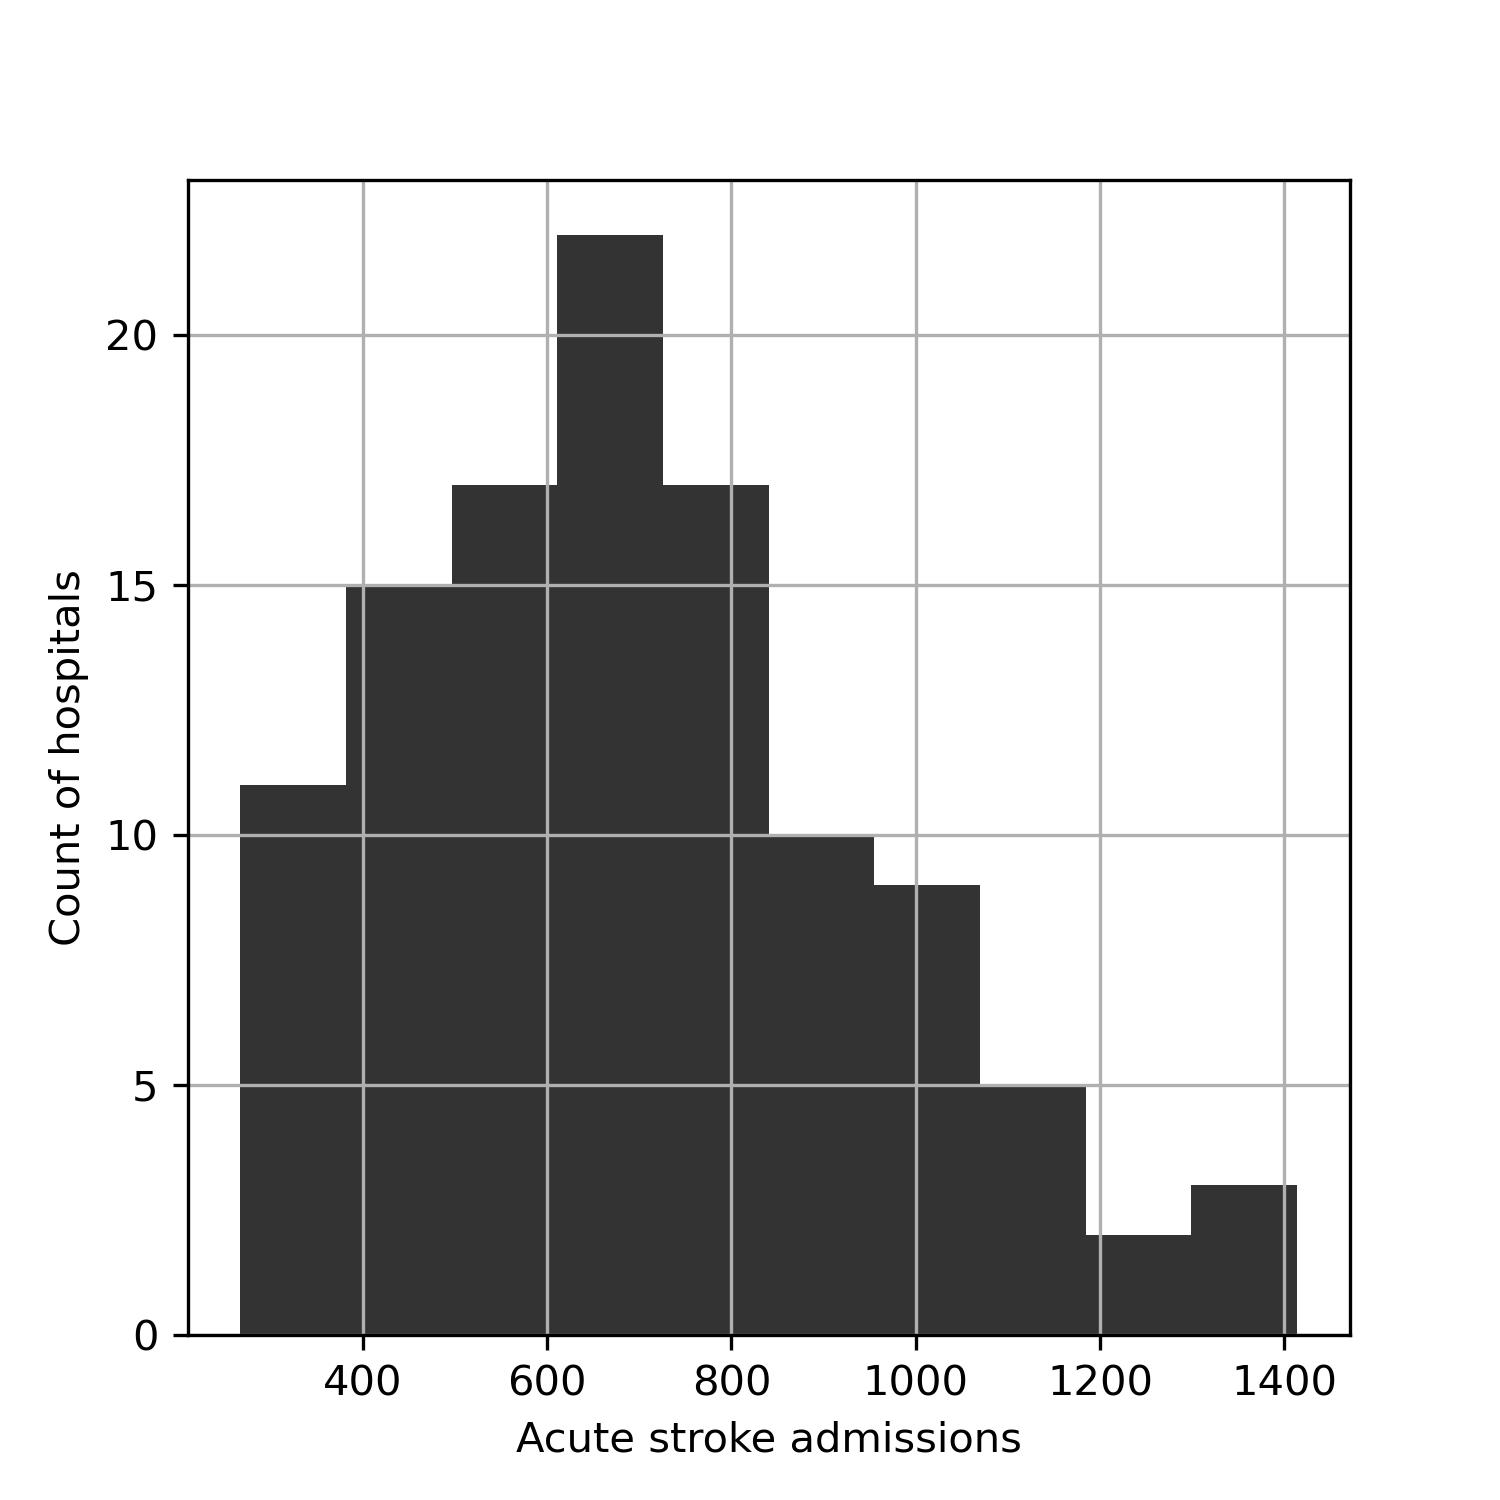
\includegraphics[width=0.95\linewidth]{./images/000_ssnap_descriptive_stats_admissions_hist}}\\
        \caption{Admissions to each of the 111 hospitals.}
        \label{fig:admission_rate}
        \end{subfigure}%ults
    \begin{subfigure}{.5\textwidth}
      \centering
      \captionsetup{width=.9\linewidth}
        {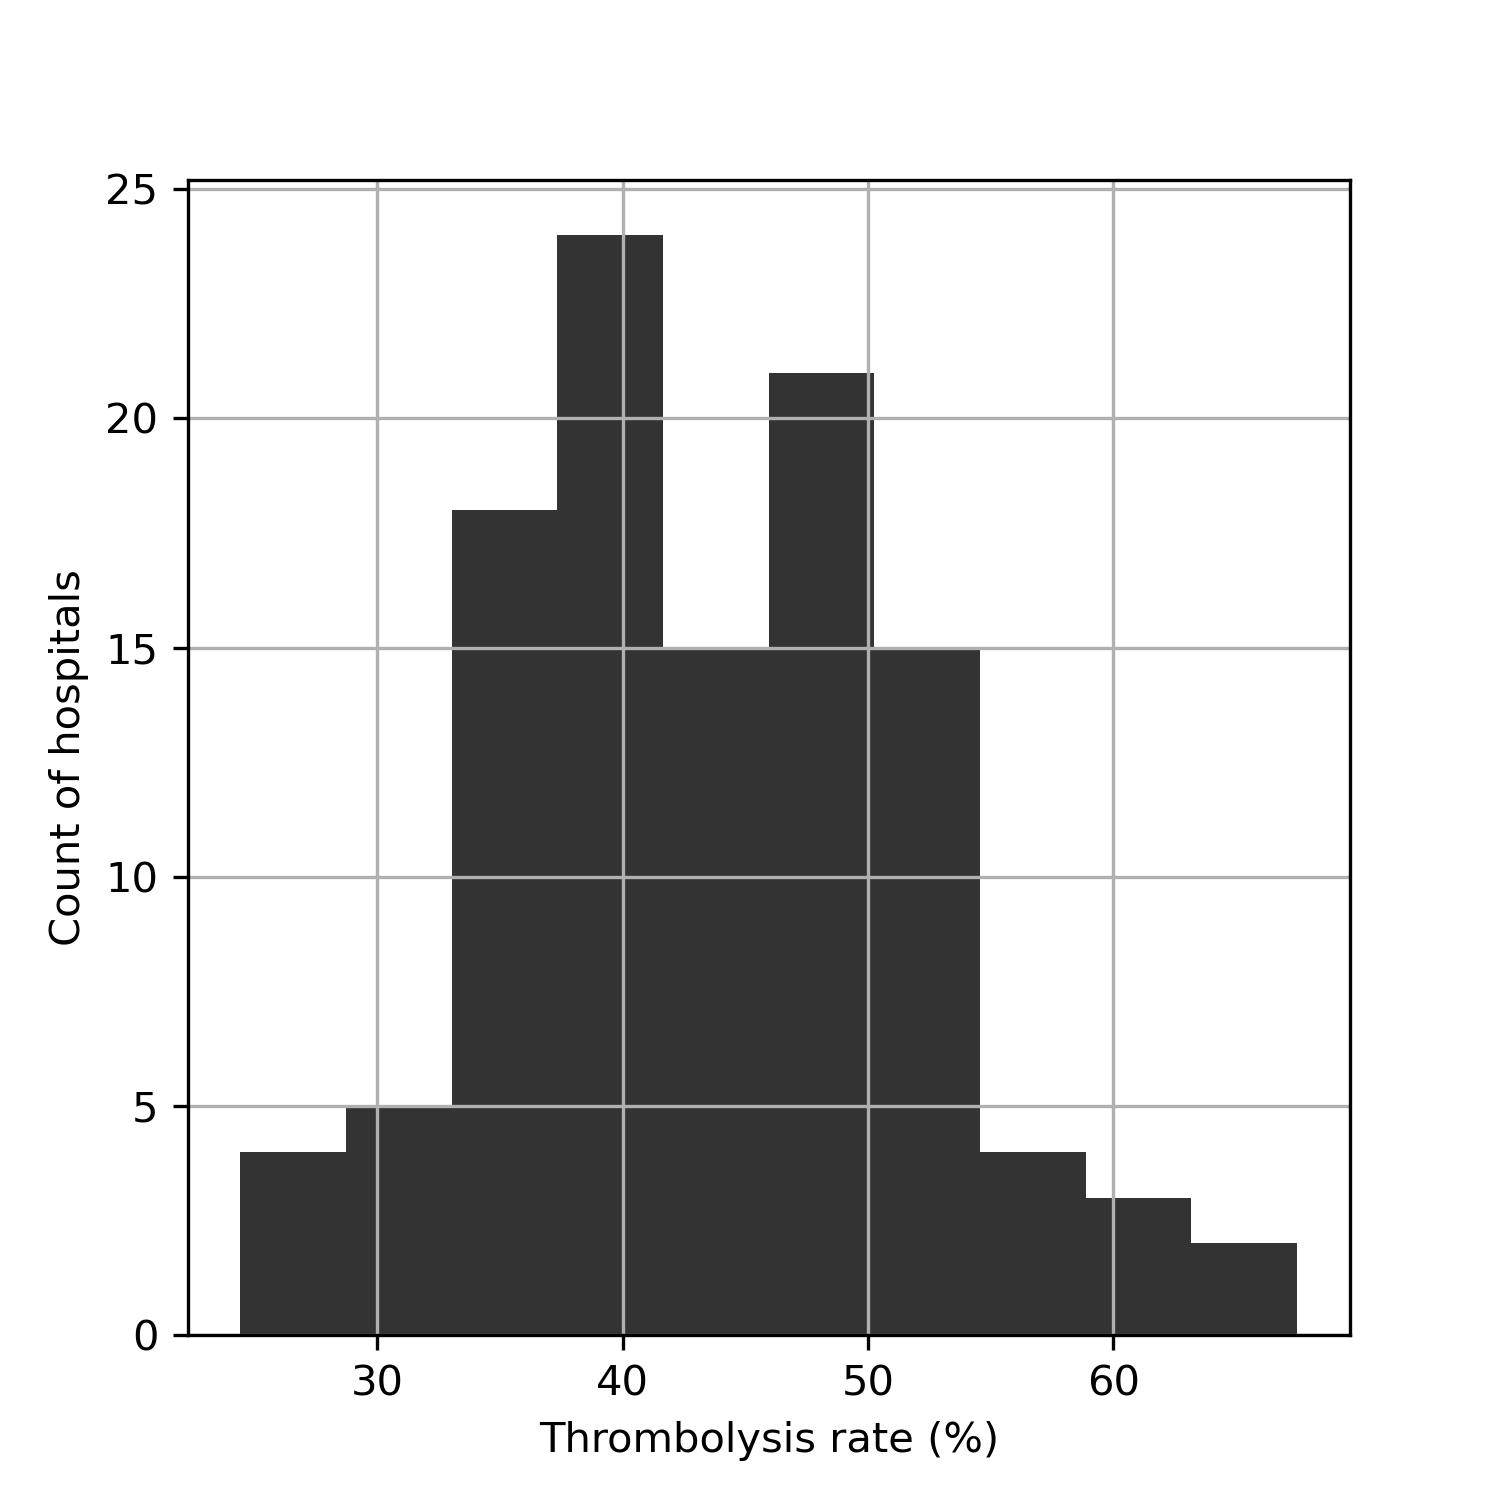
\includegraphics[width=0.95\linewidth]{./images/000_ssnap_descriptive_stats_thrombolysis_rate_hist}}\\
        \caption{Thrombolysis rate at each of the 111 hospitals}
        \label{fig:thrombolysis_rate}
    \end{subfigure}
    \caption{Histograms describing the hospitals}
\end{figure}

Figure \ref{fig:mrs_dist_wrt_ivt_bar} shows the distribution of mRS at discharge for two patient cohorts: those that receive thrombolysis, and those that do not.

\begin{figure}[h!]
    \centering
    {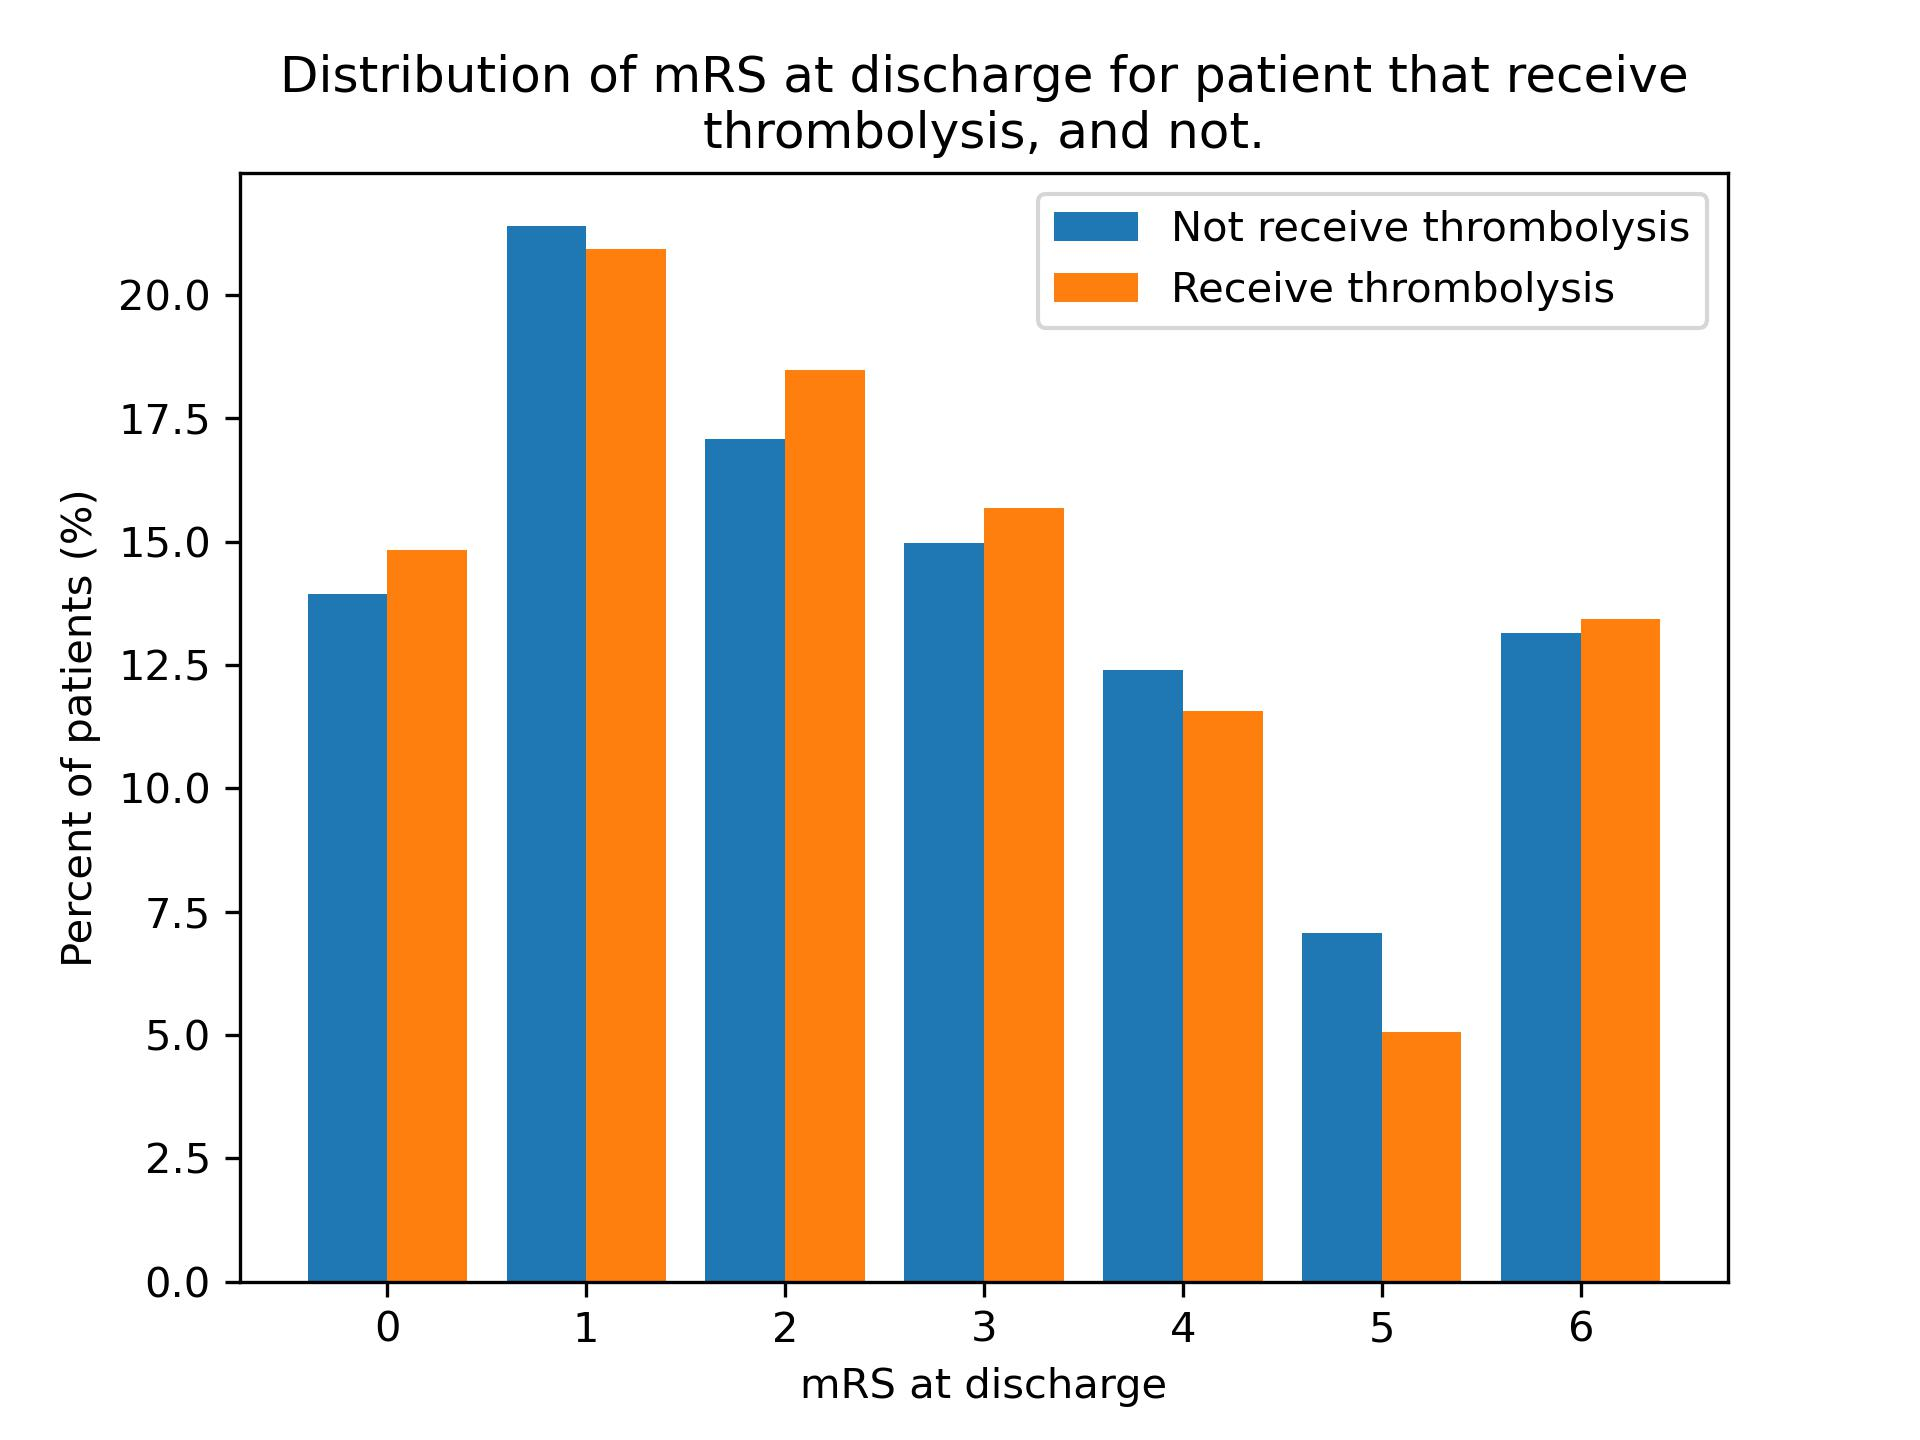
\includegraphics[width = 4in]{./images/000_ssnap_descriptive_stats_mrs_distribution_wrt_ivt.jpg}}\\
    \caption{Distribution of mRS at discharge, with respect to whether receive thrombolysis, or not.}
    \label{fig:mrs_dist_wrt_ivt_bar}
\end{figure}

\subsection{Learning curve}

We trained an XGBoost multiclass classification model to predict disability at discharge using all features as input, with a fixed 25\% test set, increment the training set size to assess whether we have enough data. Results are shown in fogure \ref{fig:learning_curve}.

\begin{figure}[h!]
    \centering
    {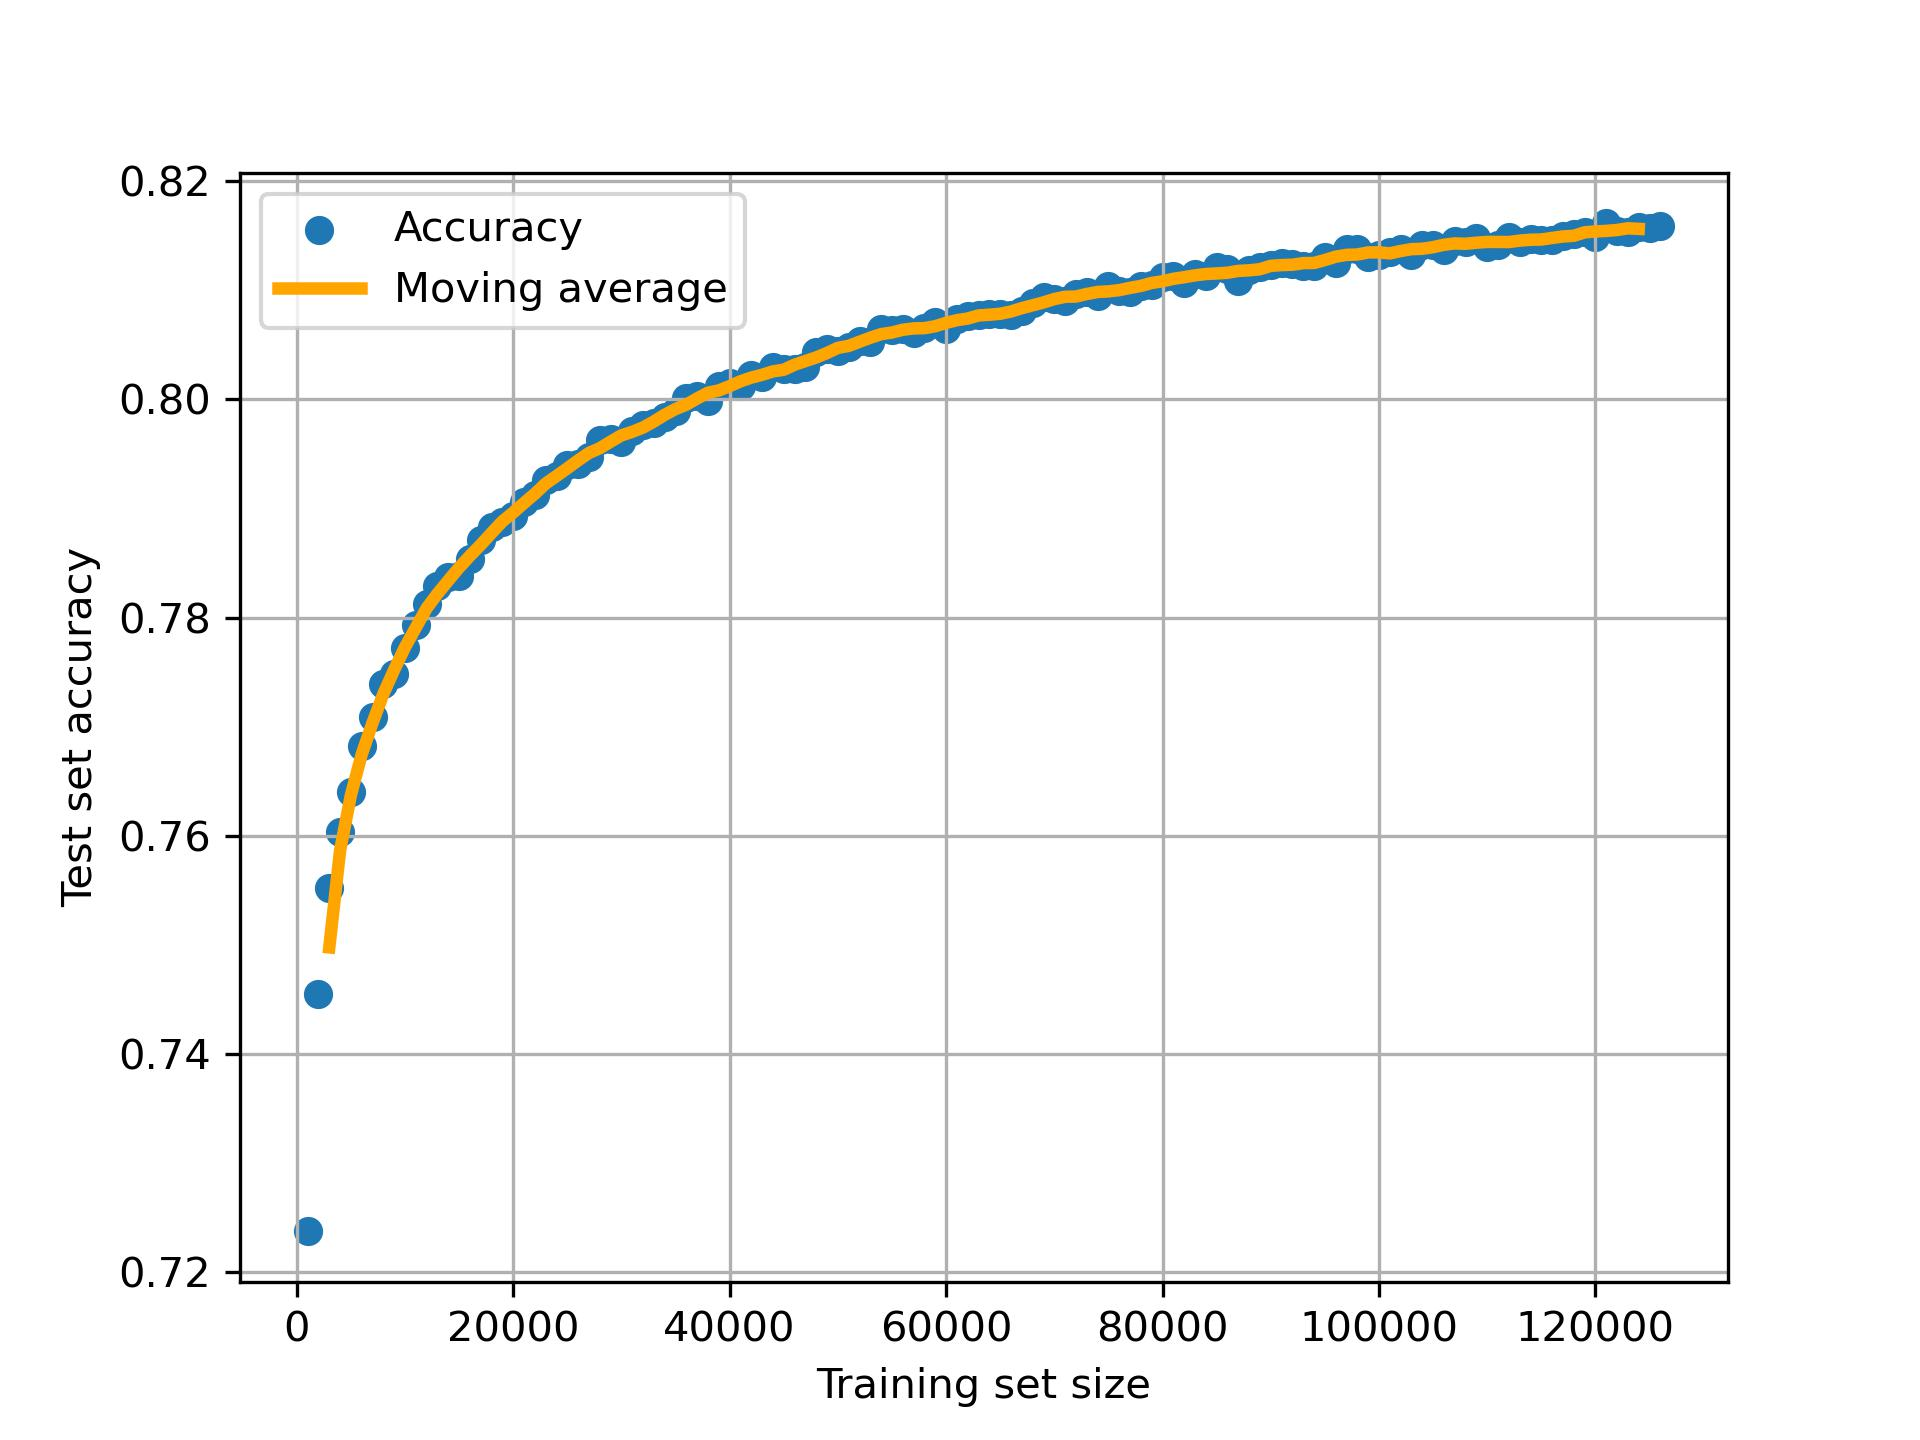
\includegraphics[width = 4in]{./images/015_xgb_all_features_learning_curve_learning_curve.jpg}}\\
    \caption{Learning rate. All features as input to the XGBoost thrombolysis outcome model (multiclass classification). Accuracy is measured as ROC-AUC.}
    \label{fig:learning_curve}
\end{figure}

\subsection{Feature selection}

Selecting which features (that describe the patients characteristics, their acute stroke pathway timings, use/time to thrombolysis, and the attended hospital) to include in an XGBoost multiclass classification model to predict disability at discharge.

\subsubsection{Model performance: All features}

The model performance with all 58 features is:
\begin{enumerate}
    \item AUC: 0.818 (std across 5 kfolds: 0.001)
    \item Accuracy: 0.440 (std across 5 kfolds: 0.002)
    \item Accuracy within one: 0.760 (std across 5 kfolds: 0.002)
\end{enumerate}

\subsubsection{Model performance: Sequentially selecting features}

Performance of models by sequentially adding the feature that incremented the performance (up to 25 features):
\begin{enumerate}
    \item prior\_disability, AUC: 0.687
    \item stroke\_severity, AUC: 0.770
    \item stroke\_team, AUC: 0.800
    \item age, AUC: 0.806
    \item year, AUC: 0.811
    \item nihss\_arrival\_loc, AUC: 0.814
    \item scan\_to\_thrombolysis\_time, AUC: 0.816
    \item thrombolysis\_no\_but\_improving, AUC: 0.817
    \item nihss\_arrival\_best\_language, AUC: 0.818
    \item new\_afib\_diagnosis, AUC: 0.818
    \item nihss\_arrival\_sensory, AUC: 0.819
    \item atrial\_fibrillation, AUC: 0.819
    \item nihss\_arrival\_facial\_palsy, AUC: 0.819
    \item thrombolysis\_no\_but\_other\_medical, AUC: 0.819
    \item infarction, AUC: 0.819
    \item arrive\_by\_ambulance, AUC: 0.819
    \item nihss\_arrival\_motor\_arm\_left, AUC: 0.819
    \item thrombolysis\_no\_but\_comorbidity, AUC: 0.819
    \item nihss\_arrival\_loc\_questions, AUC: 0.819
    \item nihss\_arrival\_motor\_arm\_right, AUC: 0.819
    \item nihss\_arrival\_best\_gaze, AUC: 0.820
    \item thrombolysis\_no\_but\_too\_mild\_severe, AUC: 0.820
    \item diabetes, AUC: 0.820
    \item thrombolysis\_no\_but\_haemorrhagic, AUC: 0.820
    \item thrombolysis\_no\_but\_medication, AUC: 0.820
\end{enumerate}

 With 15 features selected, the model choose a feature (infarction) that is the same value for all patients. We interpreted that to mean that no more information was being obtained beyond this point by adding a single feature.
 
\subsection{Feature selection - additional experiments}

To inform us further about which features to include in our model, we carried out some additional experiments. 

Here is what we learnt, and our selection of 7 features based on this:
\begin{enumerate}
    \item prior\_disability (easy selection choice)
    \item stroke\_severity (checked the impact of using the separate NIHSS features instead - decided including stroke severity captured the information)
    \item stroke\_team (easy selection choice)
    \item age (easy selection choice)
    \item onset\_to\_thrombolysis\_time (scan\_to\_thrombolysis\_time is a selected feature, however the feature onset-to-thrombolysis time is a more useful feature to include as it aligns with other research and the clinical focus.We compared the SHAP plots from models that included either (and neither) of these duration features. Across the three models, the other features (age, prior disability, stroke severity) are not affected by the inclusion of either duration feature, nor is any performance accuracy lost)
    \item any\_afib\_diagnosis (Both new\_afib\_diagnosis and atrial\_fibrillation featrures are in the list above, and we have seen that an atrial fibrillation diagnosis contributes for the mRS6 outcome. We will include any\_afib\_diagnosis as this includes both of the other atrial fibrillation features information. We compared the SHAP plots from models that included one of these atrial fibrillation diagnosis features (and none). Across those models, the other features (age, prior disability, stroke severity) are not affected by the inclusion of which atrial fibrillation feature, nor is any performance accuracy lost).
    \item precise\_onset\_known (Not included in the feature selection list, however may be useful to include so people can see whether it makes a significant difference to outcomes, as this is often a discussion point amongst clinicians)
\end{enumerate}

\textbf{Why we didn't include these features:}
\begin{enumerate}
    \item YEAR: Any data from beyond 2021 (the latest year in the dataset), the model has yet to see any information about that year. If the decision tree treats the ”Year” feature as a numerical value, any future year will be grouped along with year 2021 for each split - check how the model is treating the Year feature.
    
    We reran feature selection excluding the feature "stroke team" as an option. 
    
    First here's the model performance of all the features, but not stroke team (56 features):
    \begin{enumerate}
        \item AUC: 0.786 (std across 5 kfolds: 0.001)
        \item Accuracy: 0.387 (std across 5 kfolds: 0.003)
        \item Accuracy within one: 0.734 (std across 5 kfolds: 0.003)
   \end{enumerate}

    
    
    The feature "Year" was now not a selected features. Here are those results:
    \begin{enumerate}
        \item prior\_disability, AUC: 0.687
        \item stroke\_severity, AUC: 0.770
        \item age, AUC: 0.777
        \item nihss\_arrival\_loc, AUC: 0.779
        \item scan\_to\_thrombolysis\_time, AUC: 0.780
        \item thrombolysis\_no\_but\_improving, AUC: 0.782
        \item nihss\_arrival\_best\_language, AUC: 0.783
        \item  thrombolysis\_no\_but\_other\_medical, AUC: 0.783
        \item nihss\_arrival\_sensory, AUC: 0.784
        \item nihss\_arrival\_facial\_palsy, AUC: 0.784
        \item nihss\_arrival\_limb\_ataxia, AUC: 0.784
        \item nihss\_arrival\_motor\_arm\_left, AUC: 0.785
        \item nihss\_arrival\_best\_gaze, AUC: 0.785
        \item diabetes, AUC: 0.785
        \item thrombolysis\_no\_but\_comorbidity, AUC: 0.785
        \item nihss\_arrival\_motor\_arm\_right, AUC: 0.786
        \item thrombolysis\_no\_but\_too\_mild\_severe, AUC: 0.786
        \item onset\_during\_sleep, AUC: 0.786
        \item precise\_onset\_known, AUC: 0.786
        \item atrial\_fibrillation, AUC: 0.786
        \item infarction, AUC: 0.786
        \item arrive\_by\_ambulance, AUC: 0.786
        \item nihss\_complete, AUC: 0.786
        \item prior\_stroke\_tia, AUC: 0.786
        \item nihss\_arrival\_dysarthria, AUC: 0.786
    \end{enumerate}

    To investigate the interaction between "stroke team" and "year" we created some binary models (as SHAP interaction can not be calculated for a multiclass model). This showed that ....?

    \item Individual NIHSS features are not included, as we are already including the feature stroke severity, and this is dependent on the individual NIHSS features (SHAP required features to be independant, apart from with the target feature)
    \item scan\_to\_thrombolysis\_time is being represented by the feature onset\_to\_thrombolysis\_time
    \item atrial\_fibrillation and new\_afib\_dianosis are being represented by the feature any\_afib\_diagnosis
    \item Thrombolysis\_no\_but\_improving (there is a messiness of this feature overlapping with the onset\_to\_thrombolysis\_time. We would now have two features saying that the patient does not receive IVT).
    \item Thrombolysis\_no\_but\_other\_medical (the SHAP plots show that this feature does not have a big effect on predicting the outcome).
\end{enumerate}

\subsubsection{Model performance: Seven chosen features}

The performance of a model with these seven input features is shown below:
\begin{enumerate}
    \item prior\_disability
    \item stroke\_severity
    \item stroke\_team
    \item age
    \item onset\_to\_thrombolysis\_time
    \item any\_afib\_diagnosis
    \item precise\_onset\_known
\end{enumerate}

\begin{enumerate}
    \item AUC: 0.809 (std across 5 kfolds): 0.001)
    \item Accuracy: 0.429 (std across 5 kfolds: 0.001)
    \item Accuracy within one: 0.746 (std across 5 kfolds: 0.002)
\end{enumerate}

\section{\textit{Multiclass outcome} model: Accuracy}

Figure \ref{fig:feature_selection} shows the mean ROCAUC for the 5 kfold model, sequentially selecting the features.

\begin{figure}[!h]
    \centering
    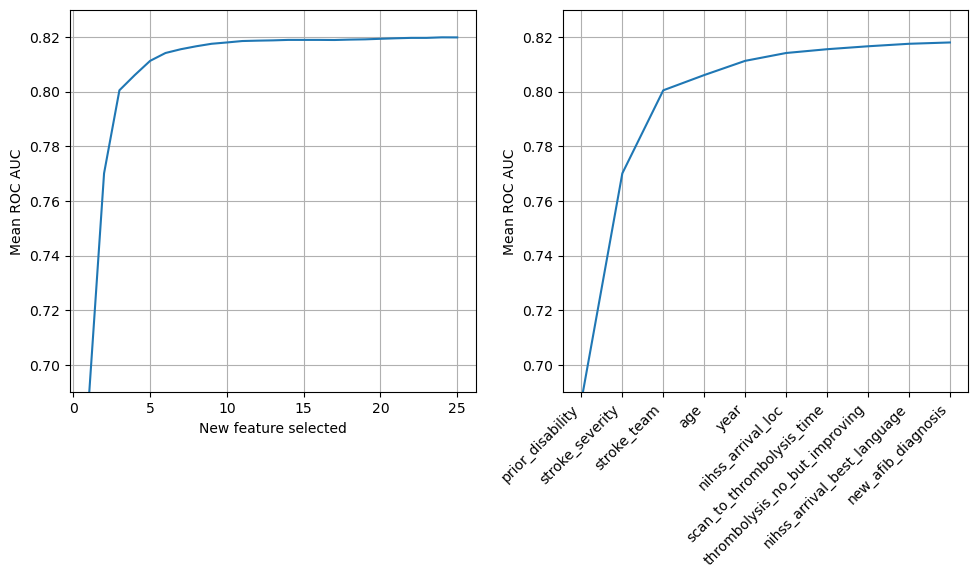
\includegraphics[width=0.75\textwidth]{./images/020_feature_selection.jpg}\\
    \caption{Feature selection}
    \label{fig:feature_selection}
\end{figure}

Figure \ref{fig:confusion_rocauc} shows the ROC-AUC results for the individual one vs one classes. There's is a better performance for classes to be distiguishable when they are further from each other in value. 

\begin{figure}[h!]
    \centering
    {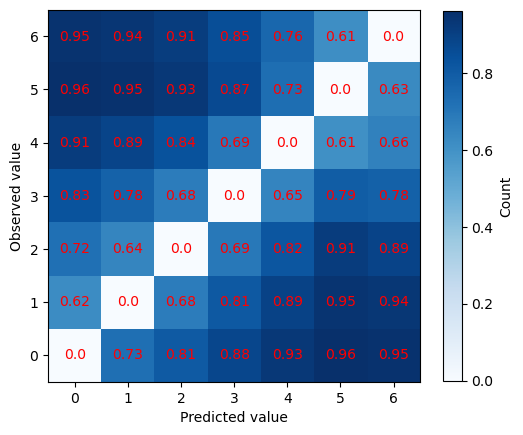
\includegraphics[width = 4in]{./images/040_ROCAUC_confusion_matrix_ovo.png}}\\
    \caption{ROC-AUC results for the individual one vs one classes}
    \label{fig:confusion_rocauc}
\end{figure}

Figure \ref{fig:confusion_mrs} shows the confusion matrices for the 5 kfolds. Given the consistency across the 5 kfolds, we will now only use results from the first kfold.
%040_confusion_matrices_5fold.png
\begin{figure}[!h]
    \centering
    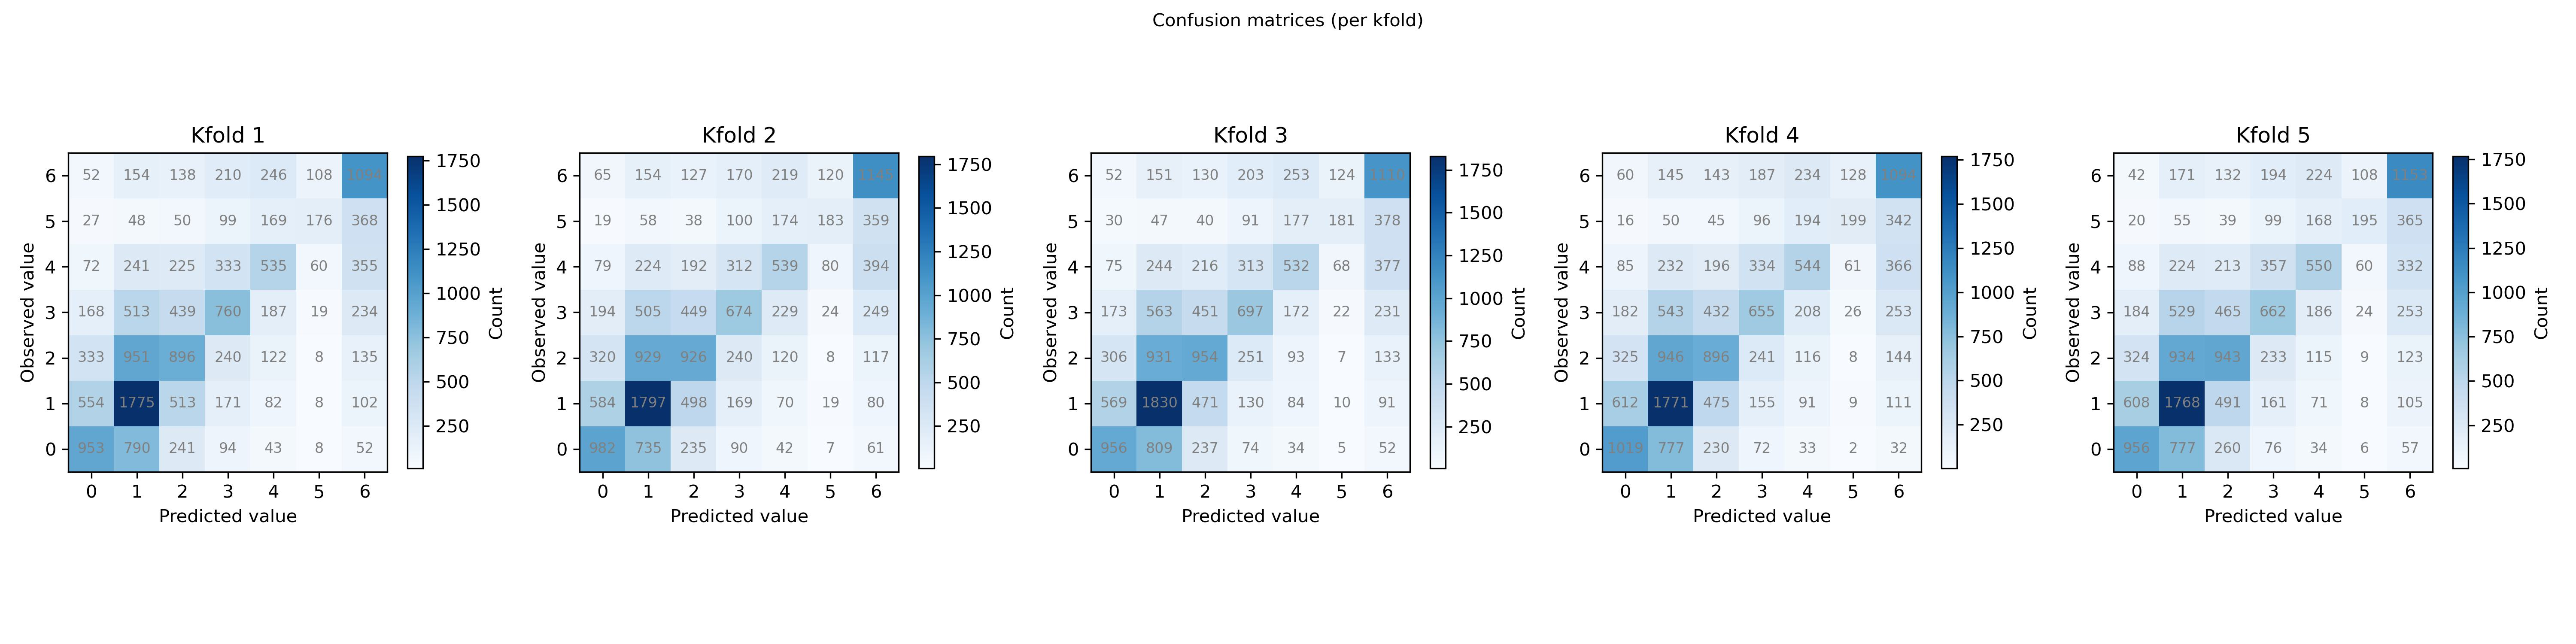
\includegraphics[width=1\textwidth]{./images/040_xgb_7_features_5fold_confusion_matrices_per_kfold.jpg}\\
    \caption{}
    \label{fig:confusion_mrs}
\end{figure}


Figure \ref{fig:violin_population_mRS} shows the outcome at population level for the different treatment scenarios.

\begin{figure}[!h]
    \centering
    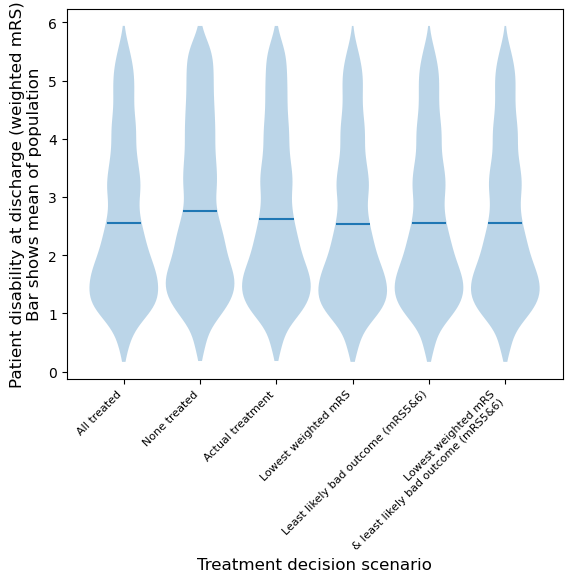
\includegraphics[width=0.7\textwidth]{./images/210_violin_population_weighted_mRS_per_treatment_scenario.png}\\
    \caption{Violin plot showing the population weighted mRS for each treatment scenario, with the bar showing the mean of the population.}
    \label{fig:violin_population_mRS}
\end{figure}


\subsection{\textit{Thrombolysis decision} model: Accuracy}

Figure \ref{fig:rocauc_thrombolysis_decision} shows the ROCAUC results for the two \textit{matching treatment} models. 


\begin{figure}
\centering
  \captionsetup{width=.9\linewidth}
  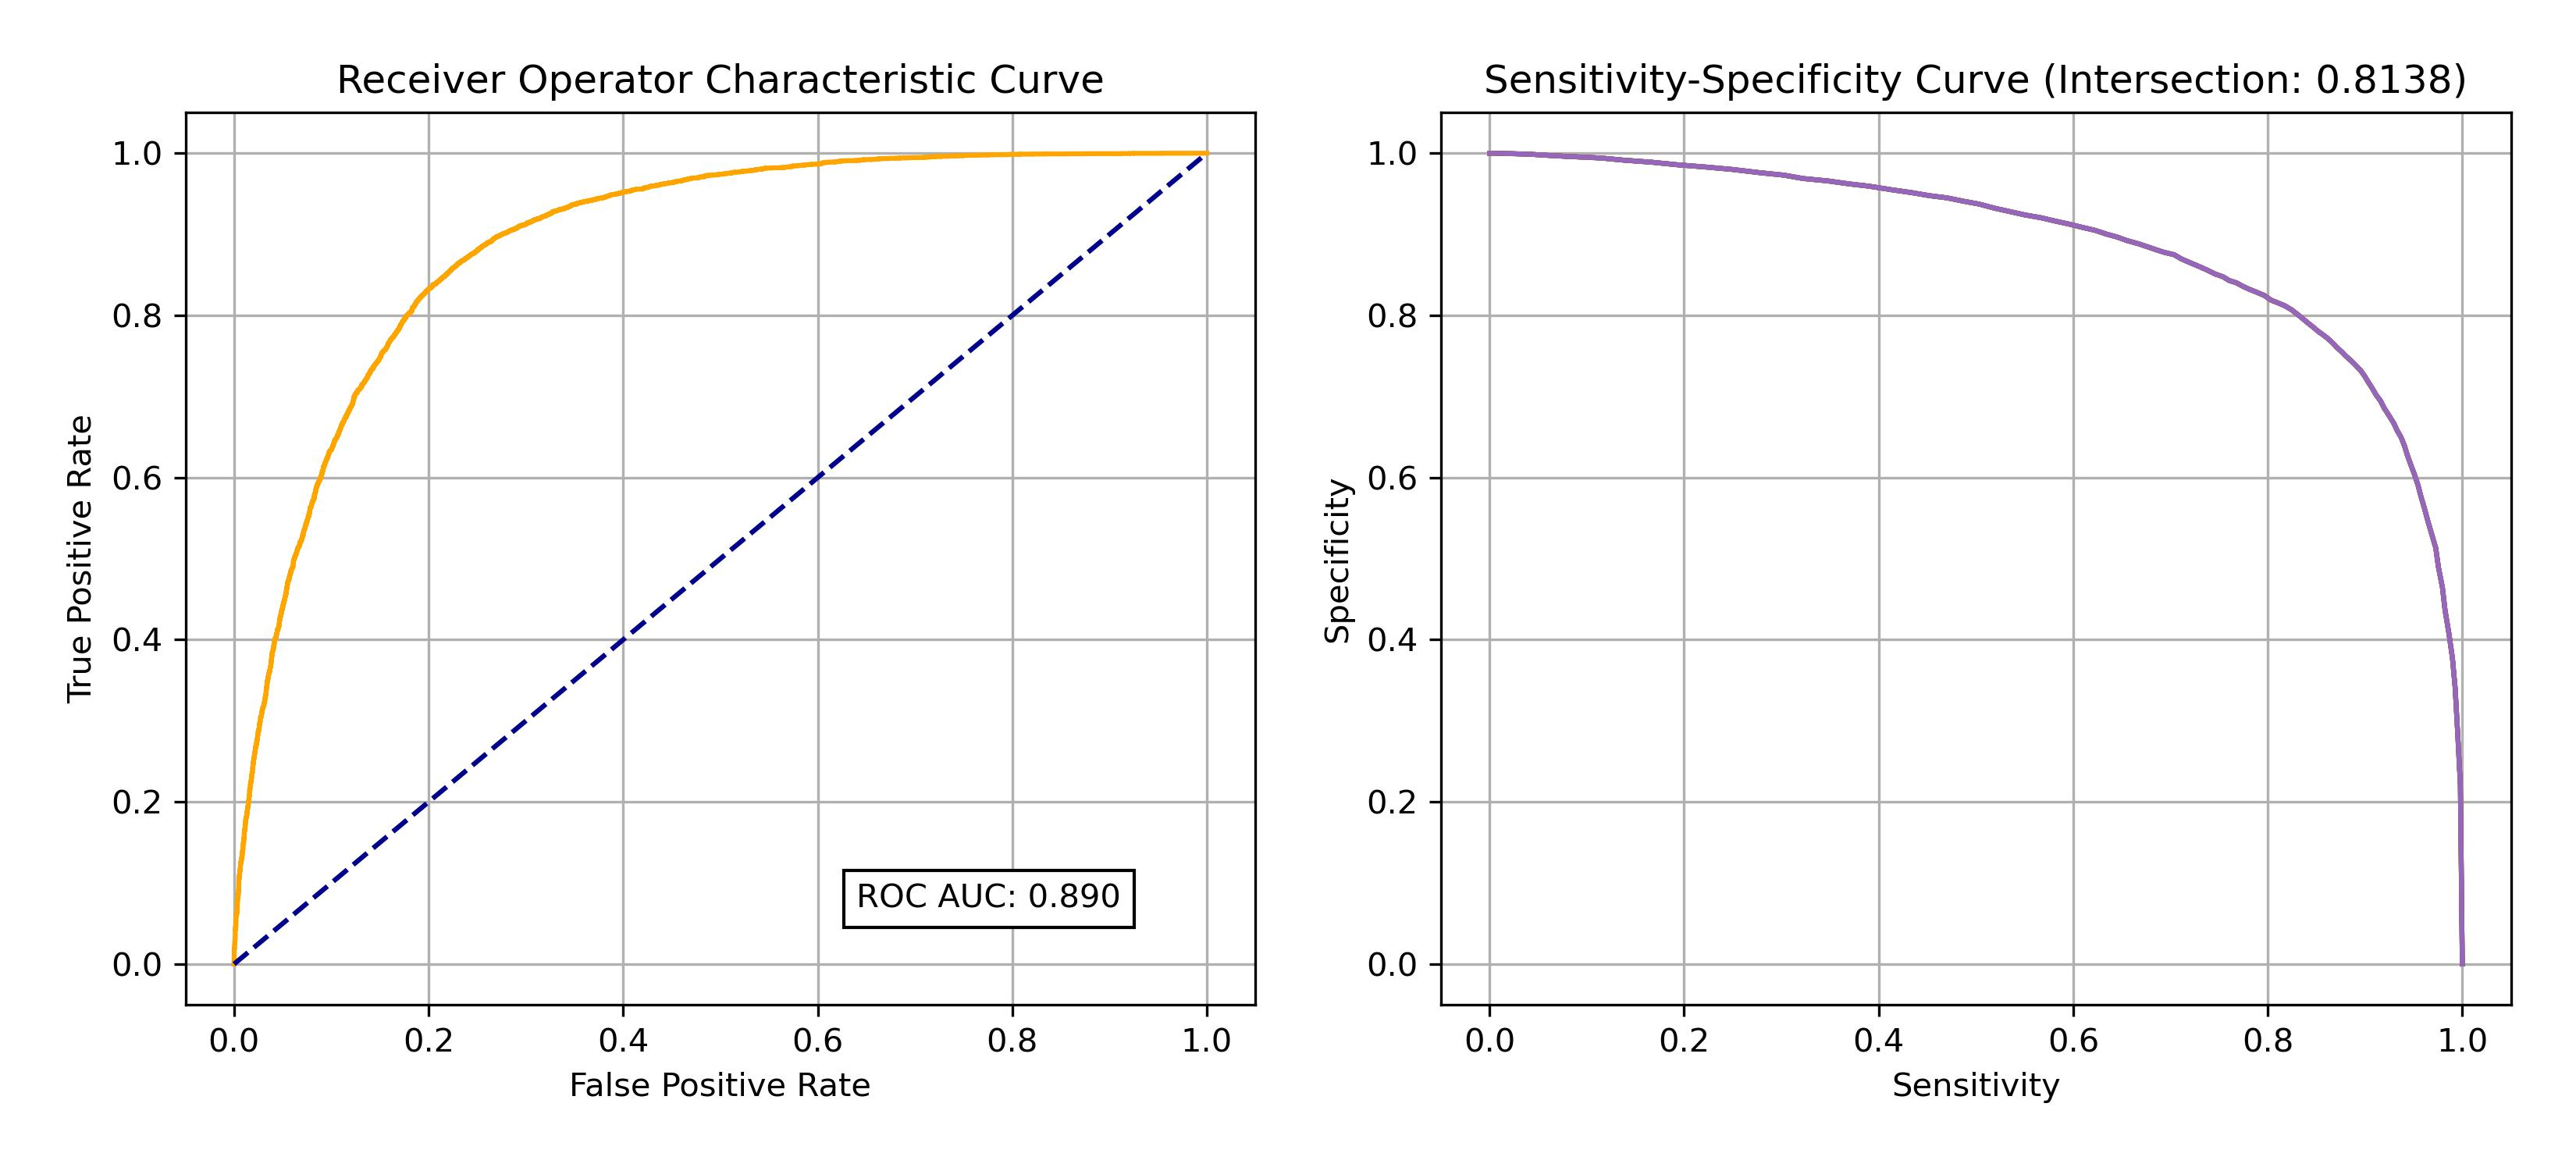
\includegraphics[width=1\textwidth]{./images/200_xgb_8_features_all_data_thrombolysis_decision_roc_sens_spec.jpg}\\
  \caption{Predicting patients receive thrombolysis (of those not have anticoagulants)}
  \label{fig:rocauc_thrombolysis_decision}
\end{figure}


\iffalse
\begin{figure}
\centering
  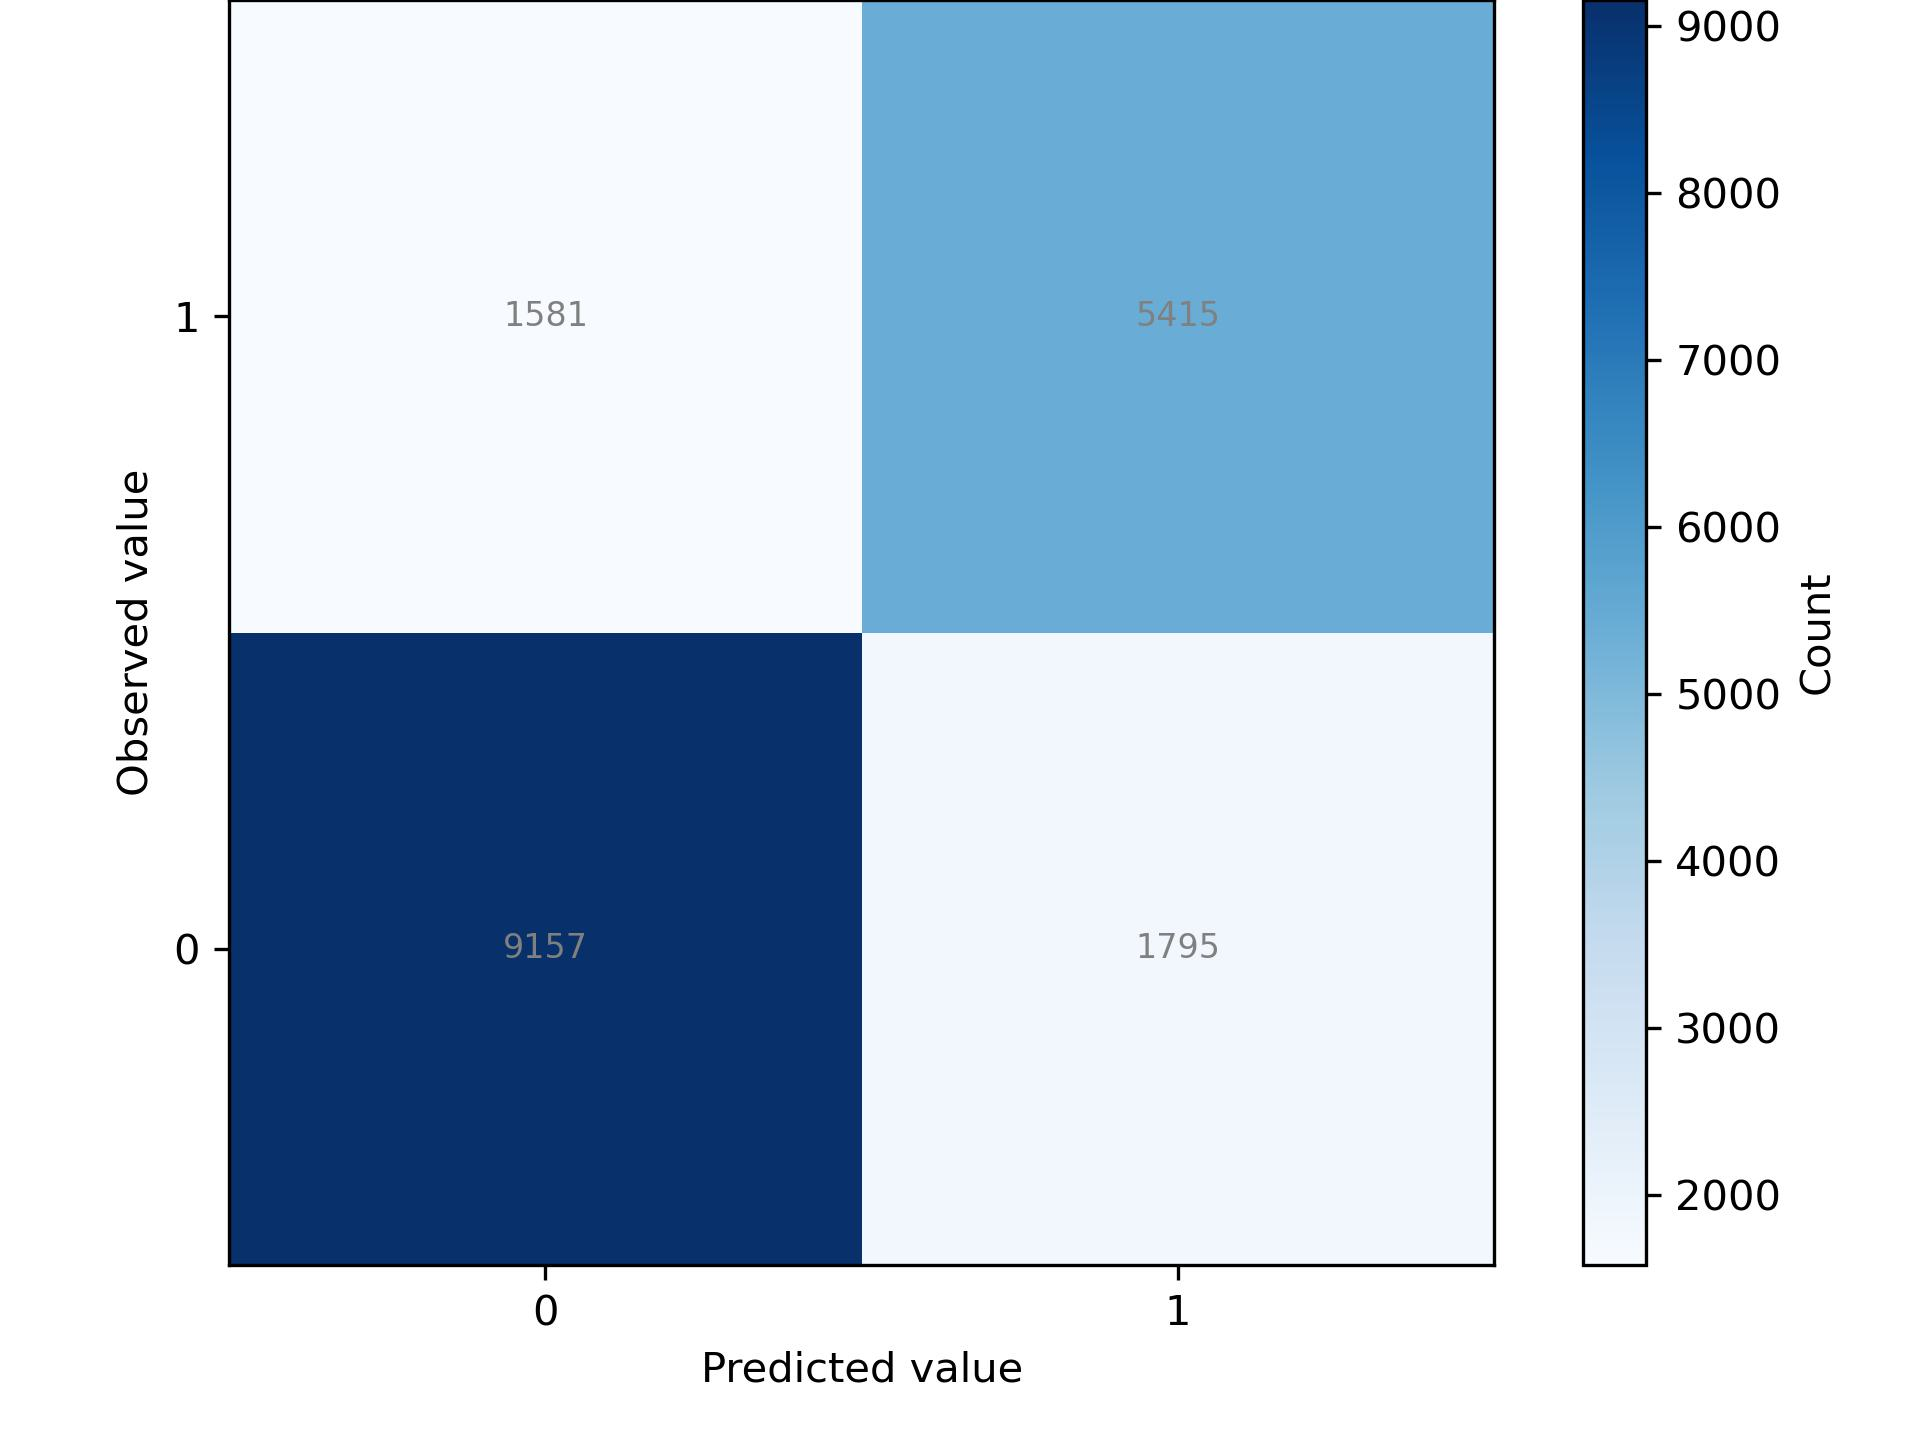
\includegraphics[width=0.6\textwidth]{./images/200_xgb_8_features_all_data_thrombolysis_decision_confusion_matrix}\\
  \caption{Predicting had treatment for those predicted to have better outcome from treatment}
  \label{fig:cm_thrombolysis_decision}
\end{figure}



\textbf{Violin plots}
Illustrate this with a violin plot. Figure \ref{fig:shap_violin_all_benefit_ivt} shows patients who should benefit from treatment. What is it about the patients that means they didn't receive it, but would have benefited from treatment?

\begin{figure}
\subfloat[]{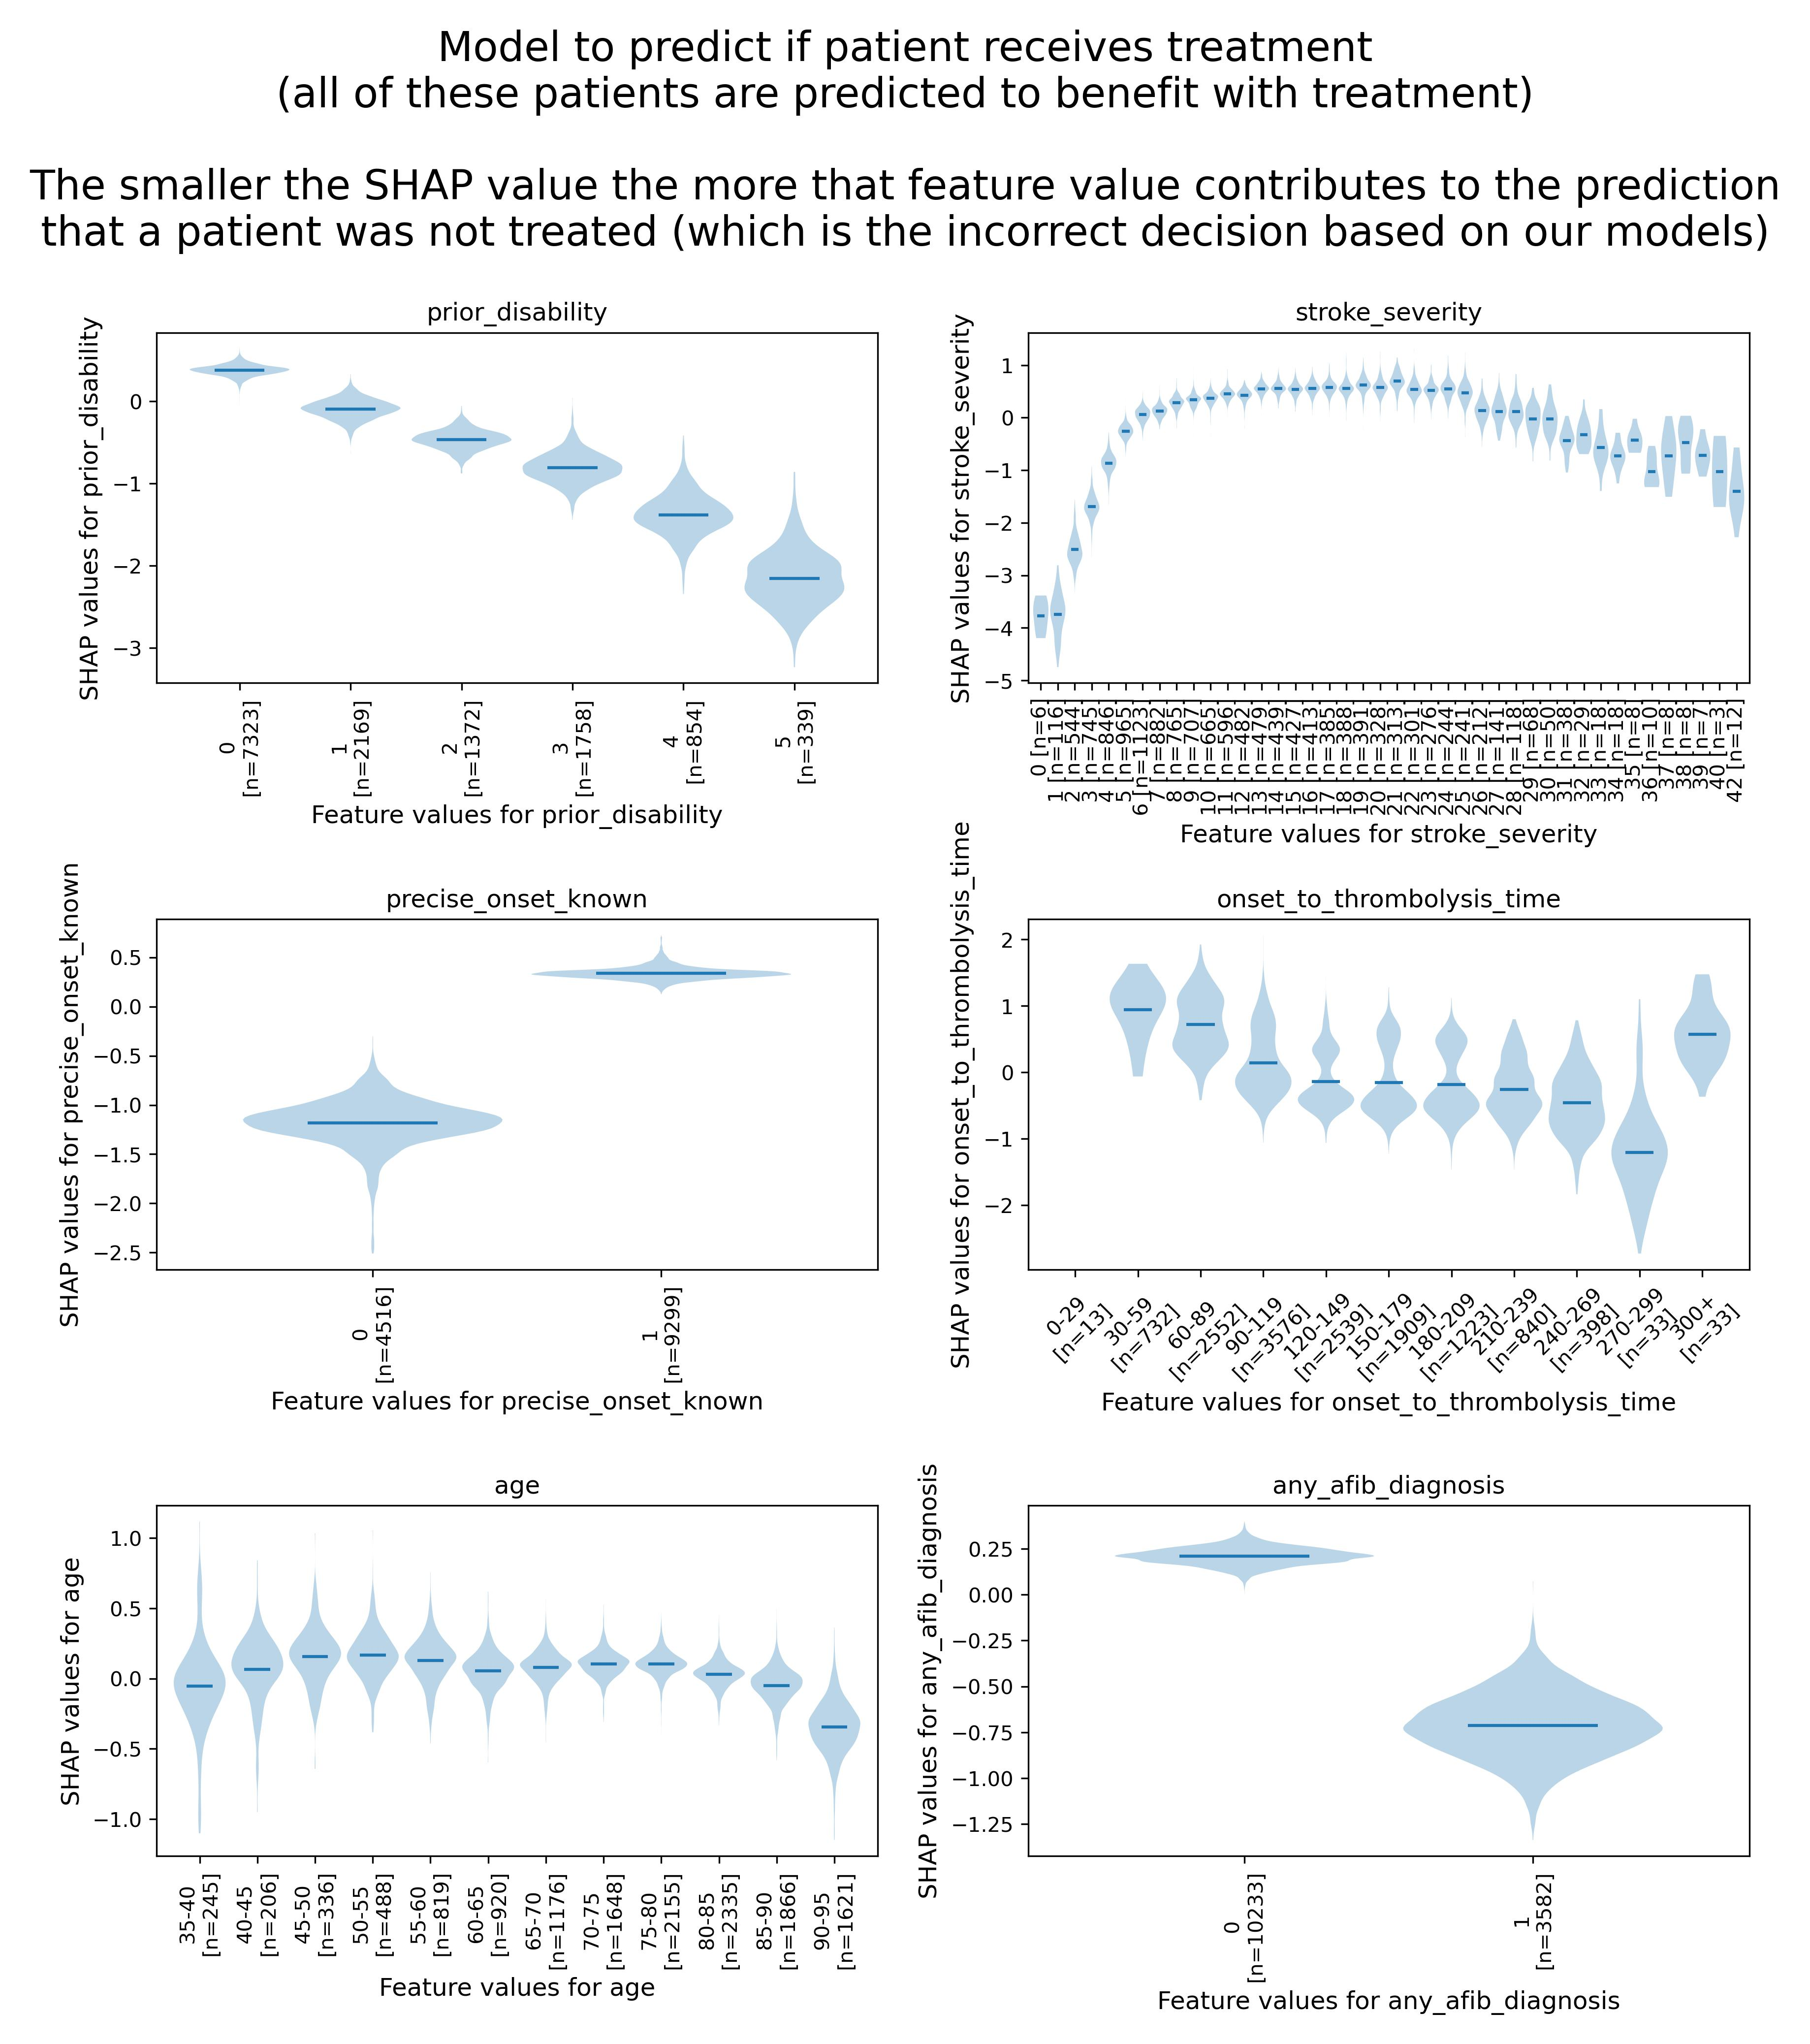
\includegraphics[width = 5in]{./images/218_shap_violin_all_benefit_with_ivt_Lowest_weighted_mrs_and_least_mrs5_6_Actual_treatment.jpg}}\\
\caption{}
\label{fig:shap_violin_all_benefit_ivt}
\end{figure}

\ref{fig:shap_violin_none_benefit_ivt} shows patients who should not benefit from treatment. What is it about the patients that means they received it, but would have benefited from not receiving treatment?

\begin{figure}
\subfloat[]{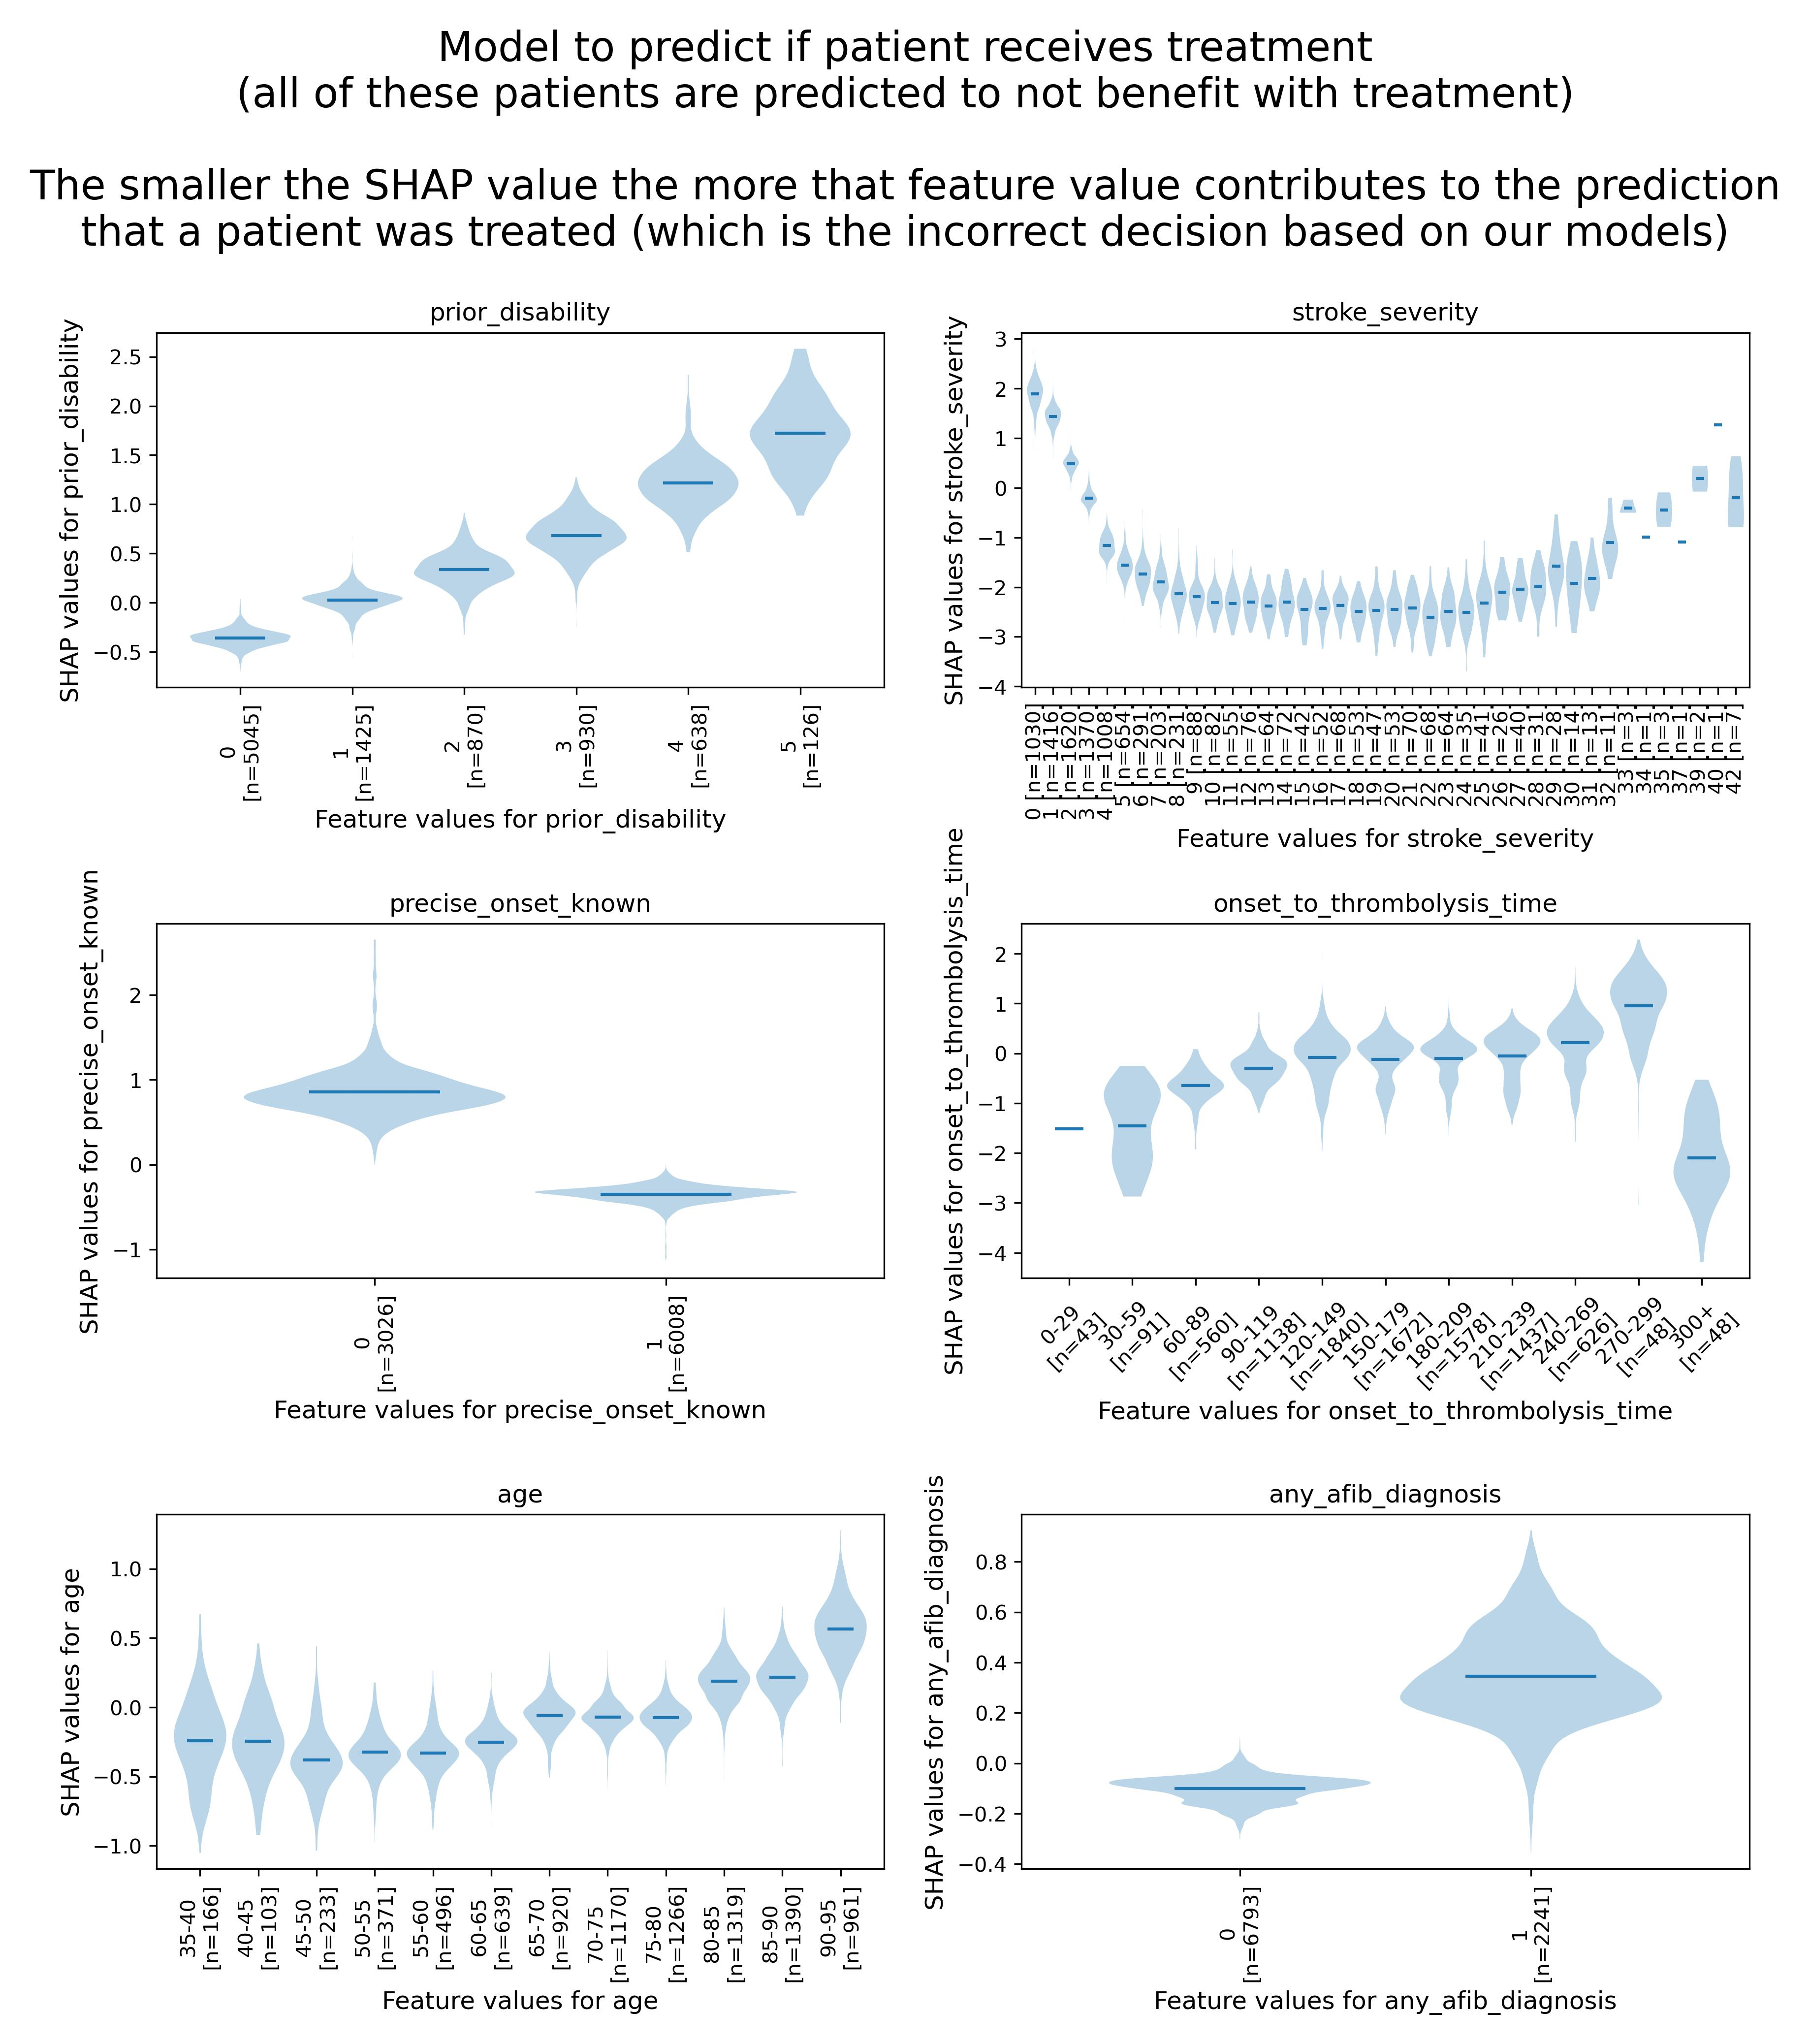
\includegraphics[width = 5in]{./images/218_shap_violin_none_benefit_with_ivt_Lowest_weighted_mrs_and_least_mrs5_6_Actual_treatment.jpg}}\\
\caption{}
\label{fig:shap_violin_none_benefit_ivt}
\end{figure}

See the points as relative, as zero means it is not shifting model from base SHAP.

Safest bet of the best outcome with treatment, choose a patient with ideal characteristics (these are younger, no AF, early IVT, SS 10-25).

These ideal characteristic values also identify patients that have been given thrombolysis but are predicted to not have the best outcome with treatment. So we can't say always give it to a single certain characteristic value, as need to take into account all characteristics.

So a drug label contains a list of ideal characteristics - if you follow this then you miss benefit. 

In order to recognise those patients who would, and would not, you need a model to combine all the characteristics. It's combination of characteristics, not a single value. No simple rules to recognise patients who should be treated but aren't currently receiving treatment (and vice versa).

On the flip side, non-ideal characteristic values (such as older, AF, later IVT, SS mild or severe) help to identify patients that have not been given thrombolysis but are predicted to have the best outcome with treatment.

All of this points back to needing a model.

The model takes into account prior disability 
\fi